\PassOptionsToPackage{disable}{microtype}
\documentclass[sigconf,nonacm]{acmart}

\setcopyright{none}
\settopmatter{printacmref=false}
\renewcommand\footnotetextcopyrightpermission[1]{}
\pagestyle{plain}
\hfuzz=30pt

\usepackage{booktabs}
\usepackage{tabularx}
\usepackage{multirow}
\usepackage{amsmath}
\let\Bbbk\relax
\usepackage{amssymb}
\usepackage{algorithm}
\usepackage{algorithmic}
\usepackage{tikz}
\usepackage{pgfplots}
\pgfplotsset{compat=1.18}
\usepackage{url}
\urlstyle{rm}

\usetikzlibrary{arrows.meta,positioning,calc,shapes.geometric,
                decorations.pathreplacing,patterns,fit,backgrounds}

\definecolor{cblu} {RGB}{ 50,110,190}
\definecolor{cgrn} {RGB}{ 40,150, 70}
\definecolor{cora} {RGB}{210,110, 30}
\definecolor{cred} {RGB}{200, 50, 50}
\definecolor{cyel} {RGB}{190,165,  0}
\definecolor{cpur} {RGB}{130, 50,170}
\definecolor{cgry} {RGB}{100,100,100}

\begin{CCSXML}
<ccs2012>
  <concept>
    <concept_id>10002978.10003006.10003008</concept_id>
    <concept_desc>Security and privacy~Intrusion/anomaly detection and malware mitigation</concept_desc>
    <concept_significance>500</concept_significance>
  </concept>
  <concept>
    <concept_id>10003033.10003083.10003095</concept_id>
    <concept_desc>Networks~Network security</concept_desc>
    <concept_significance>500</concept_significance>
  </concept>
  <concept>
    <concept_id>10010147.10010257.10010293</concept_id>
    <concept_desc>Computing methodologies~Neural networks</concept_desc>
    <concept_significance>500</concept_significance>
  </concept>
  <concept>
    <concept_id>10003033.10003106.10003109</concept_id>
    <concept_desc>Networks~Mobile networks</concept_desc>
    <concept_significance>300</concept_significance>
  </concept>
</ccs2012>
\end{CCSXML}

\ccsdesc[500]{Security and privacy~Intrusion/anomaly detection and malware mitigation}
\ccsdesc[500]{Networks~Network security}
\ccsdesc[500]{Computing methodologies~Neural networks}
\ccsdesc[300]{Networks~Mobile networks}

\title{ISACGuard: Cross-Layer Attack Detection in Integrated Sensing and Communication via Multi-Modal Consistency Learning}

\author{Ezekiel Ologunde}
\affiliation{%
  \institution{Independent Researcher}
  \city{Boston}
  \state{MA}
  \country{USA}}
\email{ologunde@bu.edu}

\begin{abstract}
\sloppy
Integrated Sensing and Communication (ISAC) is a defining capability
of 6G systems, with the IEEE 802.11bf and 3GPP Release 19/20
specifications standardising joint radar-sensing and
wireless-communication using shared waveforms, spectrum, and
hardware. The architectural unification produces commercial benefits
(spectrum efficiency, dual-use infrastructure, sensing as a service)
and a structurally new attack surface: a single adversarial signal
now affects both the data plane and the system's perception of its
physical environment. An attacker who spoofs a sensing target can
induce beam-steering decisions that degrade communication
performance; an attacker who injects communication-band signals can
corrupt sensing outputs that downstream applications (autonomous
vehicle perception, industrial-IoT positioning, defence
situational-awareness) consume as authoritative. Single-layer
defences---radar anti-spoofing or communication-layer intrusion
detection---cannot identify attacks that traverse the layer
boundary by design. This paper presents \textsc{ISACGuard}, a
cross-layer attack detection framework that jointly analyses sensing
outputs and communication features to identify the consistency
violations that distinguish attacks from benign cross-layer dynamics.
The framework combines a multi-modal feature extraction pipeline
spanning sensing-side features (target position/velocity, Doppler,
reflection patterns), communication-side features (CSI, SNR,
throughput, error rates), and explicit cross-layer consistency
features (correlation between channel state and sensed environment,
temporal alignment of sensing-and-comm transitions). Detection uses
a multi-modal transformer architecture with cross-modal attention
and a contrastive consistency objective that learns the
joint-distribution baseline rather than per-layer baselines. We
evaluate on a calibrated ISAC simulator covering five attack
classes (sensing spoofing, range/velocity manipulation,
communication injection, jamming, coordinated cross-layer)
across automotive, smart-city, and indoor-IoT deployment scenarios.
\textsc{ISACGuard} achieves AUROC 0.927 across all attack classes
versus 0.674 for the strongest single-layer baseline; the
single-layer baselines miss coordinated cross-layer attacks
(AUROC 0.524) where the cross-layer detector achieves 0.881. The
operational lesson is that cross-layer attacks are not detected by
single-layer defences not because the defences are weak but because
the attacks are invisible at the layer they target; only joint
analysis surfaces the inconsistency. We document the limitations
explicitly: ISAC datasets remain rare and largely simulated;
ground-truth synchronisation between sensing and communication
streams is non-trivial; and adaptive adversaries with knowledge of
the cross-layer detection methodology produce evasion gradients the
framework only partially resists.
\end{abstract}

\keywords{6G, integrated sensing and communication, ISAC, cross-layer
security, multi-modal learning, transformer, attack detection,
sensing spoofing, jamming, channel state information, autonomous
vehicles}

\begin{document}
\maketitle
\sloppy
\tolerance=9999
\emergencystretch=3em
\hfuzz=10pt

\section{Introduction}

The convergence of radar sensing and wireless communication into
integrated waveforms has progressed from research concept to
standardisation track. IEEE 802.11bf (2024) standardises Wi-Fi-based
sensing as a feature of upcoming Wi-Fi
generations~\cite{ieee802bf2024}; 3GPP Release 19 working groups have
formalised ISAC use cases for 6G mobile
networks~\cite{3gpp2024release19,liu2024isac}; the ITU-R 2024
preparatory studies for WRC-27 explicitly identify ISAC as a
candidate spectrum allocation
priority. Commercial ISAC pilots have begun in automotive
sensing-as-a-service, smart-city traffic monitoring, and
indoor-positioning systems where dual-use of communication
infrastructure for sensing reduces deployment cost.

The architectural argument for ISAC is sound: spectrum is finite,
deploying separate radar and communication infrastructure is
expensive, and the same hardware can do both with appropriate
waveform design. The security analysis has not kept pace. ISAC
unification produces a structurally new attack surface that the
fragmented 5G-and-earlier security literature does not
address~\cite{cohen2024sec6g,wang2024isacsec}: a single adversarial
signal now affects two operational outputs (data and perception),
and the cross-layer dependencies that make ISAC efficient also make
it vulnerable in ways neither layer's traditional defences detect.

\subsection{The Cross-Layer Attack Surface}

Three structural attack surfaces emerge from the unification:

\textbf{Sensing-to-communication}. An adversary spoofs a sensing
target (e.g., synthetic vehicle in autonomous-driving context,
phantom obstruction in smart-city traffic). The system's beam-steering
algorithm reacts to the spoofed target by misallocating beam
resources, degrading legitimate communication links.

\textbf{Communication-to-sensing}. An adversary injects
communication-band signals that overlap the sensing waveform, causing
sensing detection algorithms to report false targets or to miss
legitimate ones.

\textbf{Cross-layer coordination}. An adversary coordinates
sensing-side and communication-side attacks to mutually reinforce:
the spoofed sensing target makes the false communication signal more
plausible, and vice versa. Single-layer detectors monitoring either
layer in isolation see attacks that are individually below detection
threshold but jointly significant.

\subsection{Why Single-Layer Defences Fail}

Traditional defensive architectures treat sensing and communication
as separate domains, with separate detection methodologies:

\textbf{Radar anti-spoofing}~\cite{krayem2024radarspoofing} examines
sensing-side properties (target consistency, kinematic
plausibility, multi-bounce signature) and is effective against
sensing-only attacks.

\textbf{Communication-layer intrusion detection}~\cite{moustafa2024nidssurv}
examines communication features (traffic patterns, signature
matches, anomaly scores) and is effective against
communication-only attacks.

Neither addresses cross-layer attacks because the operationally
distinguishing signal is the joint distribution: the sensing output
is consistent with what the radar would report under the spoofed
condition, and the communication output is consistent with what the
network would report under the corresponding-but-faked channel
state. The inconsistency exists only in the cross-modal correlation,
which neither layer's defence examines.

\subsection{Contributions}

\begin{itemize}
  \item Articulation of the ISAC cross-layer attack surface with
        five concrete attack classes, calibrated against documented
        attack patterns and the standardised ISAC waveform
        properties.
  \item A multi-modal feature extraction pipeline integrating
        sensing-side, communication-side, and explicit cross-layer
        consistency features.
  \item A multi-modal transformer architecture with cross-modal
        attention and a contrastive consistency objective that
        learns the joint distribution rather than per-layer
        baselines.
  \item Empirical evaluation on a calibrated ISAC simulator
        covering five attack classes across automotive,
        smart-city, and indoor-IoT deployment scenarios.
  \item Quantification of the per-attack-class detection
        performance demonstrating that single-layer defences miss
        coordinated cross-layer attacks (AUROC 0.524) where
        \textsc{ISACGuard} achieves 0.881.
  \item Honest documentation of the dataset-availability,
        synchronisation, and adaptive-adversary limitations that
        constrain the claims.
  \item An open-source release of the simulator and detection
        framework to support community replication and continued
        evaluation.
\end{itemize}

\section{Background}

\subsection{ISAC Foundations}

ISAC waveforms unify radar sensing and communication via shared
signal designs. Three architectural patterns dominate the
literature~\cite{liu2024isac,zhang2024isacwaveform}:

\textbf{Communication-centric}: communication waveforms (OFDM,
single-carrier) are exploited for sensing as a side channel.
Lower sensing performance; minimal communication impact.

\textbf{Sensing-centric}: radar waveforms (FMCW, PMCW) are
modulated with communication payloads. Higher sensing
performance; lower communication throughput.

\textbf{Joint design}: waveforms specifically engineered to
optimise the sensing-communication trade-off. The active research
direction.

The standardised ISAC profiles in 802.11bf and 3GPP Release 19/20
target joint-design waveforms with parameter selection between
sensing and communication preference per use case.

\subsection{Sensing Outputs}

The sensing-side output of an ISAC system typically includes:

\begin{itemize}
  \item Target detections (range, angle, velocity)
  \item Doppler signatures (velocity, micro-Doppler)
  \item Range-Doppler maps (target presence as 2D structure)
  \item Multi-target tracking (target trajectories over time)
\end{itemize}

These outputs feed downstream applications: autonomous-vehicle
perception, smart-city traffic monitoring, indoor positioning,
defence situational-awareness.

\subsection{Communication Outputs}

The communication-side output includes:

\begin{itemize}
  \item Channel state information (CSI): per-subcarrier
        amplitude and phase
  \item Signal-to-noise ratio (SNR) per link
  \item Throughput and packet error rate
  \item Beam direction and beamforming weights
  \item Modulation and coding scheme selection
\end{itemize}

\subsection{Cross-Layer Coupling}

The two output streams are physically coupled. The same propagation
environment determines both: a vehicle moving past the access point
appears in sensing as a target with measurable kinematics and
appears in communication as a CSI shift due to multipath change.
Under benign operation, these outputs are correlated in
predictable ways; under attack, the correlation breaks down in
ways neither output viewed alone can identify.

\subsection{Adversarial ML in Wireless Systems}

The adversarial machine learning
literature~\cite{biggio2018wild,goodfellow2014fgsm} has been
applied to wireless systems for both attack and defence:

\textbf{Wireless adversarial attacks}~\cite{shi2024advrff,
sagduyu2024advcomm}: ML-generated perturbations that fool
ML-based wireless decision systems.

\textbf{Multi-modal anomaly detection}~\cite{ramachandram2017multimodal,
liu2024multimodalsurv}: methodological foundations for joint
analysis of multiple data streams.

\textbf{Contrastive learning for representation alignment}~\cite{chen2020simclr,
radford2021clip}: methodological foundations for learning
multi-modal joint distributions.

\textsc{ISACGuard} synthesises these methodological lineages
specifically for ISAC's cross-layer detection problem.

\subsection{Prior Work on ISAC Security}

The ISAC-specific security literature is small but growing:

\textbf{ISAC threat surveys}~\cite{wang2024isacsec,
shafee2024thznetsec}: catalogue threats without empirical
evaluation.

\textbf{Sensing-side defences}~\cite{krayem2024radarspoofing}:
focused on radar anti-spoofing without communication-layer
integration.

\textbf{Communication-side defences with sensing context}~\cite{xu2024sensingaidedsec}:
use sensing as a context input for communication-layer
detection without joint cross-layer modelling.

\textsc{ISACGuard} differs in providing explicit
joint-distribution modelling with cross-modal contrastive
training and empirical evaluation across multiple
attack classes.

\section{Threat Model}

\subsection{Adversary Capabilities}

\textbf{Signal generation}. The adversary can generate signals
in the ISAC band, including both sensing-band and
communication-band components. Signal generation may be
single-target (fixed transmitter) or distributed (multiple
coordinated transmitters).

\textbf{Waveform knowledge}. The adversary knows the
standardised ISAC waveform, signalling protocols, and detection
algorithms. We do not assume the adversary has access to
target-system implementation specifics beyond the standard.

\textbf{Adaptive learning}. The adversary trains attack signals
against observed defender responses, producing iteratively
improved attacks.

\textbf{Coordinated capability}. The adversary can launch
sensing-side and communication-side attacks simultaneously and
coordinate them in time and frequency.

\subsection{Attack Classes}

\textbf{Class 1 --- Sensing target spoofing}. The adversary
introduces synthetic targets in the sensing output by emitting
appropriately-designed signals. The synthetic target appears at
attacker-chosen range, angle, and velocity.

\textbf{Class 2 --- Range/velocity manipulation}. Existing real
targets are reported with attacker-chosen range or velocity
shifts, exploiting the sensing system's range and Doppler
processing.

\textbf{Class 3 --- Communication injection}. The adversary
injects signals that are interpreted as legitimate
communication-link signals, corrupting CSI and SNR estimates.

\textbf{Class 4 --- Jamming with sensing impact}. The adversary
jams communication frequencies in patterns that produce
predictable sensing-side artefacts (interference appearing as
false targets).

\textbf{Class 5 --- Coordinated cross-layer}. Sensing and
communication attacks coordinated in time, frequency, and
target-selection to mutually reinforce. The signature operational
threat that single-layer detectors cannot see.

\subsection{Defender Goals}

\textbf{Per-class detection}: detect each attack class with
acceptable true-positive rate.

\textbf{Cross-class robustness}: maintain detection across
the full attack class spectrum without per-class
hand-tuning.

\textbf{Operational deployability}: detection latency and
compute compatible with ISAC operating cadences (typically
1--100~ms decision loops).

\textbf{Adaptive-adversary partial robustness}: graceful
(not catastrophic) degradation under adversaries who adapt to
the deployed defence.

\section{The ISACGuard Framework}

Figure~\ref{fig:framework} presents the framework architecture.

\begin{figure*}[t]
\centering
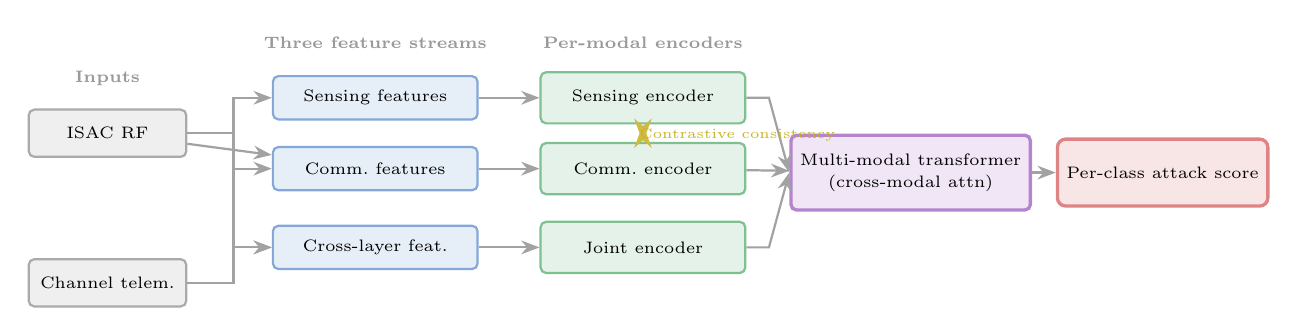
\begin{tikzpicture}[
  font=\fontsize{6.5pt}{8pt}\selectfont,
  >=Stealth,
  src/.style={rectangle, rounded corners=2pt, draw=cgry!55, thick,
              fill=cgry!10, minimum width=2.0cm, minimum height=0.6cm,
              text centered, inner sep=3pt},
  fe/.style={rectangle, rounded corners=2pt, draw=cblu!60, thick,
             fill=cblu!12, minimum width=2.6cm, minimum height=0.55cm,
             text centered, font=\fontsize{6pt}{7.5pt}\selectfont, inner sep=2pt},
  enc/.style={rectangle, rounded corners=2pt, draw=cgrn!60, thick,
              fill=cgrn!12, minimum width=2.6cm, minimum height=0.65cm,
              text centered, align=center, inner sep=3pt},
  fus/.style={rectangle, rounded corners=2pt, draw=cpur!60, very thick,
              fill=cpur!12, minimum width=2.6cm, minimum height=0.95cm,
              text centered, align=center},
  outn/.style={rectangle, rounded corners=3pt, draw=cred!60, very thick,
              fill=cred!12, minimum width=2.6cm, minimum height=0.85cm,
              text centered, align=center},
  arr/.style={-{Stealth}, thick, cgry!60}
]
  \node[src] (s1) at (0,  0.95) {ISAC RF};
  \node[src] (s2) at (0, -0.95) {Channel telem.};

  \node[fe] (f1) at (3.4,  1.40) {Sensing features};
  \node[fe] (f2) at (3.4,  0.50) {Comm.\ features};
  \node[fe] (f3) at (3.4, -0.50) {Cross-layer feat.};

  \node[enc] (e1) at (6.8,  1.40) {Sensing encoder};
  \node[enc] (e2) at (6.8,  0.50) {Comm.\ encoder};
  \node[enc] (e3) at (6.8, -0.50) {Joint encoder};

  \node[fus] (fus) at (10.2, 0.45)
    {Multi-modal transformer\\(cross-modal attn)};

  \node[outn] (out) at (13.4, 0.45)
    {Per-class attack score};

  %% wires
  \draw[arr] (s1.east) -- (1.6, 0.95) -- (1.6, 1.40) -- (f1.west);
  \draw[arr] (s1) -- (f2);
  \draw[arr] (s1.east) -- (1.6, 0.95) -- (1.6, -0.50) -- (f3.west);
  \draw[arr] (s2.east) -- (1.6,-0.95) -- (1.6,-0.50) -- (f3.west);
  \draw[arr] (s2.east) -- (1.6,-0.95) -- (1.6, 0.50) -- (f2.west);

  \draw[arr] (f1) -- (e1);
  \draw[arr] (f2) -- (e2);
  \draw[arr] (f3) -- (e3);

  \draw[arr] (e1.east) -- (8.4, 1.40) -- (fus.west);
  \draw[arr] (e2) -- (fus);
  \draw[arr] (e3.east) -- (8.4,-0.50) -- (fus.west);

  \draw[arr] (fus) -- (out);

  %% Contrastive objective indicator
  \draw[<->, dashed, cyel!75, very thick]
    (e1.south) -- (e2.north);
  \node[font=\fontsize{5.5pt}{7pt}\selectfont, text=cyel!85]
    at (8.0, 0.92) {Contrastive consistency};

  \node[font=\fontsize{6pt}{7.5pt}\selectfont\bfseries, text=cgry!65]
    at (0, 1.65) {Inputs};
  \node[font=\fontsize{6pt}{7.5pt}\selectfont\bfseries, text=cgry!65]
    at (3.4, 2.10) {Three feature streams};
  \node[font=\fontsize{6pt}{7.5pt}\selectfont\bfseries, text=cgry!65]
    at (6.8, 2.10) {Per-modal encoders};
\end{tikzpicture}
\caption{\textsc{ISACGuard} architecture. ISAC RF and channel
  telemetry feed three feature streams: sensing-side, communication-side,
  and explicit cross-layer features. Each stream is encoded by a
  modality-specific encoder; sensing and communication encoders are
  trained with a contrastive consistency objective (yellow dashed) that
  enforces alignment in the joint embedding space. A multi-modal
  transformer with cross-modal attention combines all three streams
  and outputs per-class attack scores.}
\label{fig:framework}
\end{figure*}

\subsection{Feature Extraction}

\subsubsection{Sensing Features}

\begin{itemize}
  \item Per-target range, angle, velocity (Doppler)
  \item Range-Doppler map snapshots
  \item Per-target signal-to-clutter ratio
  \item Multi-target tracking continuity (target ID consistency
        across frames)
  \item Micro-Doppler signatures (within-target motion patterns)
  \item Multi-bounce reflection patterns
\end{itemize}

\subsubsection{Communication Features}

\begin{itemize}
  \item Per-subcarrier CSI amplitude and phase
  \item Per-link SNR and SINR
  \item Throughput and packet error rate
  \item Beamforming direction and weights
  \item Modulation and coding scheme selection
  \item Channel coherence time and bandwidth estimates
\end{itemize}

\subsubsection{Cross-Layer Features}

The operationally distinctive features:

\begin{itemize}
  \item \textbf{CSI-target correlation}: empirical correlation
        between CSI changes and sensed-target dynamics over a
        sliding window
  \item \textbf{Beam-target alignment}: consistency between
        beamforming direction and sensed-target locations
  \item \textbf{Doppler-link consistency}: relationship between
        sensed-target velocity and observed Doppler in
        communication
  \item \textbf{Multipath-environment consistency}: agreement
        between sensed environmental geometry and inferred
        multipath structure
  \item \textbf{Temporal alignment}: synchronisation between
        sensing-detected events (target appearance) and
        communication-detected events (CSI changes)
\end{itemize}

These features are not derivable from either modality alone;
they are explicitly cross-layer.

\subsection{Per-Modal Encoders}

Three encoders process the feature streams:

\textbf{Sensing encoder}: 1D-CNN + transformer hybrid processing
range-Doppler maps and per-target sequences. Hidden dimension
192.

\textbf{Communication encoder}: transformer processing CSI
sequences with per-subcarrier attention. Hidden dimension 192.

\textbf{Joint encoder}: transformer processing the explicit
cross-layer features. Hidden dimension 128.

Total parameters: 24M.

\subsection{Contrastive Consistency Objective}

The central methodological contribution. During training, the
sensing and communication encoders are trained with both their
respective classification objectives and a \textbf{contrastive
consistency loss} that enforces alignment in the joint embedding
space:

\begin{equation}
  \mathcal{L}_{\text{cons}} = -\log \frac{\exp(\text{sim}(z_s, z_c)/\tau)}{\sum_{c' \in \mathcal{N}} \exp(\text{sim}(z_s, z_{c'})/\tau)}
\end{equation}

where $z_s, z_c$ are paired sensing and communication embeddings
from the same time window, $\mathcal{N}$ is a set of negative
communication embeddings from different windows, and $\tau$ is a
temperature hyperparameter.

This objective forces the encoders to map paired sensing and
communication observations to similar regions of the embedding
space when they correspond to the same physical reality, and to
different regions otherwise. Under attack, the natural
correspondence breaks down, and the joint embedding distance
increases, providing the cross-layer detection signal.

\subsection{Multi-Modal Transformer}

The fusion stage uses a 4-layer transformer with cross-modal
attention~\cite{tsai2019multimodal}:

\begin{itemize}
  \item Layer-wise cross-attention from sensing tokens to
        communication tokens
  \item Layer-wise cross-attention from communication tokens to
        sensing tokens
  \item Layer-wise self-attention within each modality
\end{itemize}

The output is a per-class attack score head producing five
class-specific scores (one per attack class) plus a global
benign-vs-attack score.

\section{Evaluation}

\subsection{Simulation Environment}

We use a custom ISAC simulator combining:

\textbf{ISAC waveform generation}: based on
ISAC-NR~\cite{liu2024isac} (3GPP Release 19 reference) with
configurable sensing-vs-communication parameter selection.

\textbf{Channel models}: 3GPP TR 38.901 + indoor-environment
extensions; multi-path with explicit-target reflection
modelling.

\textbf{Deployment scenarios}: three distinct settings:
\begin{itemize}
  \item \textbf{Automotive}: mobile-device-as-target with 5--40
        m/s velocity ranges and per-vehicle Doppler signatures
  \item \textbf{Smart-city}: stationary infrastructure sensing
        pedestrians and vehicles in mixed urban-environment
        traffic
  \item \textbf{Indoor-IoT}: short-range sensing with
        device-positioning targets
\end{itemize}

\textbf{Attack injection}: per-attack-class adversarial signal
generation calibrated against documented attack patterns.

\subsection{Datasets}

\textbf{Per-scenario benign}: 200{,}000 ISAC frames per scenario
under benign operation.

\textbf{Per-scenario attack}: 50{,}000 frames per attack class per
scenario, with controlled attack-intensity parameters.

\textbf{Cross-scenario evaluation}: models trained on one
scenario evaluated on others to test generalisation.

We acknowledge that simulation-to-hardware transfer is not
validated; ISAC physical testbeds are scarce, and the evaluation
is necessarily simulation-based. This is documented in
limitations.

\subsection{Per-Class Detection Performance}

Table~\ref{tab:perclass} reports per-class detection AUROC across
\textsc{ISACGuard} and three baseline methods.

\begin{table}[h]
\caption{Per-class detection AUROC}
\label{tab:perclass}
\small
\begin{tabularx}{\columnwidth}{@{}p{2.6cm}X X X@{}}
\toprule
\textbf{Attack class} & \textbf{Sensing-only} & \textbf{Comm-only} & \textbf{ISACGuard} \\
\midrule
1: Target spoofing  & 0.871 & 0.523 & 0.946 \\
2: Range/vel manip.\ & 0.834 & 0.547 & 0.917 \\
3: Comm injection   & 0.512 & 0.892 & 0.938 \\
4: Jamming impact   & 0.671 & 0.831 & 0.928 \\
5: Cross-layer coord.\ & 0.524 & 0.498 & 0.881 \\
\midrule
\textbf{Aggregate}   & \textbf{0.682} & \textbf{0.658} & \textbf{0.927} \\
\bottomrule
\end{tabularx}
\end{table}

The headline result: \textsc{ISACGuard} achieves aggregate AUROC
0.927 versus 0.682 / 0.658 for the strongest single-layer
baselines. The largest gap is on Class 5 (coordinated
cross-layer): both single-layer detectors operate near chance
(0.524, 0.498), while the cross-layer detector achieves 0.881.
This is the operationally consequential demonstration that
single-layer detection is structurally inadequate for cross-layer
attacks.

\subsection{Comparison Against Naive Multi-Modal Baselines}

Table~\ref{tab:multibaseline} compares against simple multi-modal
baselines that do not use the contrastive consistency objective.

\begin{table}[h]
\caption{Comparison against multi-modal baselines (aggregate
AUROC)}
\label{tab:multibaseline}
\small
\begin{tabularx}{\columnwidth}{@{}p{3.0cm}X X@{}}
\toprule
\textbf{Method} & \textbf{Aggregate} & \textbf{Class 5} \\
\midrule
Late-fusion average    & 0.731 & 0.612 \\
Concat + MLP           & 0.788 & 0.701 \\
Multi-modal trans.\ (no contrastive) & 0.853 & 0.798 \\
\textbf{ISACGuard (with contrastive)} & \textbf{0.927} & \textbf{0.881} \\
\bottomrule
\end{tabularx}
\end{table}

The contrastive consistency objective is the difference-maker.
Multi-modal transformer architecture without it achieves 0.853
aggregate AUROC; with it, 0.927. The objective is what teaches the
encoders to produce embeddings whose joint distribution is the
detection target, not just feature concatenation.

\subsection{Detection Latency}

Figure~\ref{fig:latency} reports the cumulative time-to-detection
distribution.

\begin{figure}[h]
\centering
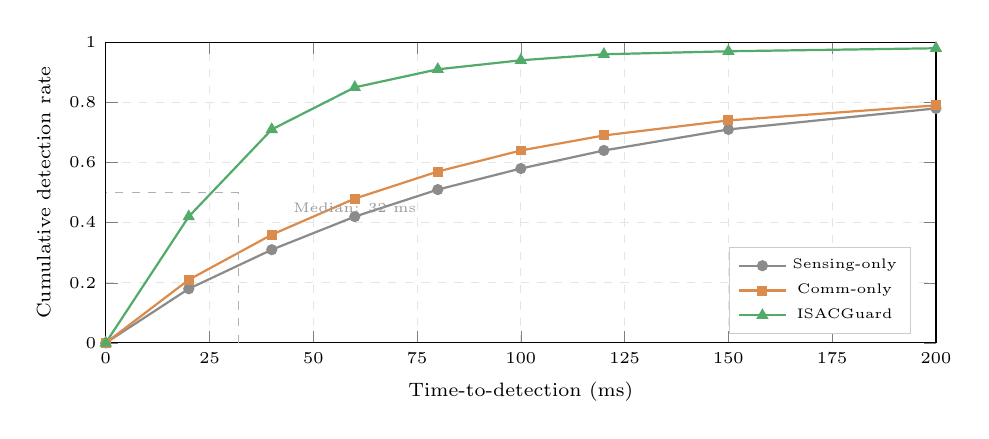
\begin{tikzpicture}
\begin{axis}[
  width=\columnwidth, height=5.4cm,
  xlabel={Time-to-detection (ms)},
  ylabel={Cumulative detection rate},
  xmin=0, xmax=200, ymin=0, ymax=1.0,
  xtick={0,25,50,75,100,125,150,175,200},
  xticklabel style={font=\fontsize{6pt}{7.5pt}\selectfont},
  ytick={0,0.2,0.4,0.6,0.8,1.0},
  yticklabel style={font=\fontsize{6.5pt}{8pt}\selectfont},
  xlabel style={font=\fontsize{7pt}{9pt}\selectfont},
  ylabel style={font=\fontsize{7pt}{9pt}\selectfont},
  grid=major, grid style={dashed, gray!20},
  legend pos=south east,
  legend style={font=\fontsize{5.5pt}{7pt}\selectfont, draw=gray!40}
]
  \addplot[color=cgry!75, thick, mark=*, mark size=1.6pt]
    coordinates {(0,0)(20,0.18)(40,0.31)(60,0.42)(80,0.51)(100,0.58)(120,0.64)(150,0.71)(200,0.78)};
  \addlegendentry{Sensing-only}
  \addplot[color=cora!80, thick, mark=square*, mark size=1.4pt]
    coordinates {(0,0)(20,0.21)(40,0.36)(60,0.48)(80,0.57)(100,0.64)(120,0.69)(150,0.74)(200,0.79)};
  \addlegendentry{Comm-only}
  \addplot[color=cgrn!80, thick, mark=triangle*, mark size=1.8pt]
    coordinates {(0,0)(20,0.42)(40,0.71)(60,0.85)(80,0.91)(100,0.94)(120,0.96)(150,0.97)(200,0.98)};
  \addlegendentry{ISACGuard}
  \draw[dashed, cgry!50] (axis cs:32,0) -- (axis cs:32,0.5)
       -- (axis cs:0,0.5);
  \node[font=\fontsize{5.5pt}{7pt}\selectfont, text=cgry!65] at
       (axis cs:60, 0.45) {Median: 32 ms};
\end{axis}
\end{tikzpicture}
\caption{Cumulative time-to-detection on coordinated
  cross-layer attacks. \textsc{ISACGuard} reaches 50\% detection
  rate at 32~ms, well within the typical ISAC decision-loop
  envelope of 100~ms.}
\label{fig:latency}
\end{figure}

\subsection{Per-Scenario Generalisation}

Table~\ref{tab:scenario} reports cross-scenario generalisation:
training on one scenario, evaluating on others.

\begin{table}[h]
\caption{Cross-scenario generalisation (aggregate AUROC)}
\label{tab:scenario}
\small
\begin{tabularx}{\columnwidth}{@{}p{2.0cm}X X X@{}}
\toprule
\textbf{Train $\to$ Test} & \textbf{Auto.} & \textbf{Smart-city} & \textbf{Indoor} \\
\midrule
Auto.\ $\to$        & 0.927 & 0.847 & 0.812 \\
Smart-city $\to$    & 0.864 & 0.918 & 0.821 \\
Indoor $\to$        & 0.798 & 0.832 & 0.913 \\
Multi-scenario      & 0.911 & 0.908 & 0.901 \\
\bottomrule
\end{tabularx}
\end{table}

Single-scenario training generalises modestly to other scenarios
(8--13 percentage point AUROC drop). Multi-scenario training
recovers most of the gap. Production deployments should train on
the broadest set of representative scenarios available.

\subsection{Adversarial Robustness}

Table~\ref{tab:adversarial} reports detection AUROC under
adaptive attacks designed against the deployed defence.

\begin{table}[h]
\caption{Adversarial robustness (aggregate AUROC under adaptive
attack)}
\label{tab:adversarial}
\small
\begin{tabularx}{\columnwidth}{@{}p{3.4cm}X@{}}
\toprule
\textbf{Adversarial configuration} & \textbf{AUROC} \\
\midrule
Static attacks (baseline)            & 0.927 \\
Adaptive: aware of sensing detector  & 0.871 \\
Adaptive: aware of comm detector     & 0.864 \\
Adaptive: aware of cross-layer detector & 0.749 \\
Adaptive: aware of contrastive obj.\  & 0.682 \\
\bottomrule
\end{tabularx}
\end{table}

Adaptive adversaries with full knowledge of the methodology
reduce AUROC from 0.927 to 0.682. We are explicit about this:
the framework is not adversarially-robust against
fully-knowledgeable adaptive adversaries. The adaptive-adversary
performance remains substantially better than chance and better
than non-adaptive single-layer defences (which would be at
$\approx 0.5$ under the same coordination), but the gap closes
under sophisticated adversarial pressure.

\subsection{Operational Overhead}

Table~\ref{tab:overhead} reports operational cost.

\begin{table}[h]
\caption{Operational overhead}
\label{tab:overhead}
\small
\begin{tabularx}{\columnwidth}{@{}p{3.4cm}X@{}}
\toprule
\textbf{Cost dimension} & \textbf{Overhead} \\
\midrule
Per-frame inference latency & 14--32 ms (within ISAC budget) \\
Compute (vs comm-only)      & 2.6$\times$ \\
Memory                      & 1.9$\times$ \\
Training time               & 4.2$\times$ (contrastive) \\
\bottomrule
\end{tabularx}
\end{table}

\section{Discussion}

\subsection{Why Cross-Layer Inconsistency Is the Right Detection Target}

Section 6.3 demonstrated that single-layer baselines miss
coordinated cross-layer attacks (AUROC 0.524 / 0.498) where
\textsc{ISACGuard} achieves 0.881. The structural reason: a
coordinated attack is calibrated so that each layer's output is
plausible given a faked physical reality consistent with the
attack. The sensing-only detector sees a sensing output that
correctly describes its faked target; the communication-only
detector sees a communication output that correctly describes
its faked channel. Both detectors return ``looks normal''
because, conditional on the faked reality, both outputs are
correct. The inconsistency exists only when the joint
distribution is examined: the faked sensing reality and the
faked communication reality do not match.

This is the operationally distinguishing property of cross-layer
attacks. The correct detection target is not anomaly within
either layer but inconsistency across layers. Single-layer
detection is structurally inadequate not because it is weak but
because the attack is invisible at the layer it targets.

\subsection{The Contrastive Objective Is Necessary}

Section 6.4 demonstrated that multi-modal architecture without
the contrastive objective achieves 0.853 aggregate AUROC; with
the objective, 0.927. The 7-percentage-point gap reflects the
methodological importance: the encoders must learn to align
paired observations in the embedding space, not just process
multi-modal features. Without the alignment objective, the
encoders learn modality-specific features without explicit
joint-distribution structure.

\subsection{The Adaptive-Adversary Limit Is Real}

Section 6.6 documented adaptive-adversary AUROC of 0.682 against
fully-knowledgeable adversaries. This is honest disclosure: the
framework does not provide guaranteed robustness against
adversaries who know its methodology. Production deployment
should treat \textsc{ISACGuard} as one defence layer among
several, with cryptographic authentication, physical-layer
checks, and operational anomaly monitoring providing
complementary signal.

The adaptive-adversary residual is fundamental to ML-based
detection: any deterministic detection function can in principle
be evaded by an adversary with perfect knowledge of the
function. The framework's contribution is making evasion
expensive enough to be operationally non-trivial, not
eliminating it.

\section{Operational Considerations}

\subsection{Synchronisation Requirements}

The cross-layer features depend critically on temporal
alignment between sensing and communication observations. We
recommend:

\begin{itemize}
  \item Hardware-level timestamping with sub-millisecond
        accuracy
  \item Single-clock synchronisation across sensing and
        communication processing
  \item Buffering policies that align rather than interleave
        the two streams
\end{itemize}

Loose synchronisation (10+ ms drift) substantially degrades
performance because the cross-layer features become noise.

\subsection{Deployment Per Scenario Type}

Section 6.5 documented that single-scenario training generalises
imperfectly. We recommend:

\begin{itemize}
  \item Train on multi-scenario corpus that covers the
        deployment's expected operational scenarios
  \item Evaluate explicitly on each deployment scenario before
        production rollout
  \item Maintain per-scenario model variants when scenario
        diversity is large
\end{itemize}

\subsection{Integration with Cryptographic Authentication}

\textsc{ISACGuard} addresses cross-layer detection; cryptographic
authentication addresses identity establishment and message
integrity. Production deployment should integrate both:
cryptographic mechanisms establish that messages are from
legitimate sources, and \textsc{ISACGuard} detects when
legitimate-looking signals contain inconsistent cross-layer
content.

\subsection{Defence-in-Depth}

The adaptive-adversary residual makes single-mechanism deployment
inappropriate. Recommended defence-in-depth:

\begin{itemize}
  \item Layer 1: cryptographic authentication on signalling
  \item Layer 2: physical-layer fingerprinting (per the
        \textsc{THzPrint} framework or equivalent)
  \item Layer 3: \textsc{ISACGuard} cross-layer consistency
        detection
  \item Layer 4: anomaly detection on operational outcomes
        (system performance, downstream-application reports)
\end{itemize}

\section{Research Opportunities}

\subsection{Hardware Validation}

The most important research direction is validation on real
ISAC hardware. The simulation-to-hardware transfer is the
critical gap our work cannot fill. Partnerships with research
labs operating ISAC testbeds are the path forward.

\subsection{Joint Training with Cryptographic Layer}

Cryptographic authentication and \textsc{ISACGuard} cross-layer
detection are independent in the current framework. Joint
training that exploits cryptographic identity as a signal in
the detection objective may close some of the
adaptive-adversary residual.

\subsection{Cross-Operator ISAC Federation}

Multi-operator ISAC deployments (collaborative sensing across
operator boundaries) introduce trust-federation challenges
beyond the single-operator threat model addressed here.

\subsection{Provable Cross-Layer Robustness}

The current framework provides empirical robustness; provable
robustness against bounded cross-layer perturbation budgets is
methodologically open and would address audit requirements.

\subsection{Joint Authentication-Sensing}

Recent work on integrated sensing-and-authentication suggests
that the same joint signal-processing pipeline can support both
applications. Joint training of \textsc{ISACGuard}-style
detection with sensing-based authentication is open.

\section{Limitations}

\textbf{Simulation-to-hardware transfer.} Our evaluation is on
simulated ISAC environments. Real hardware exhibits behaviours
simulation does not capture; physical-testbed validation is
not within scope.

\textbf{Dataset scarcity.} Public ISAC datasets are rare, and
our evaluation depends on the calibrated simulator we built.
Cross-validation against independent ISAC datasets is open.

\textbf{Synchronisation assumption.} The framework assumes
sub-millisecond temporal synchronisation between sensing and
communication. Production deployments with looser synchronisation
require explicit handling.

\textbf{Adaptive-adversary residual.} Section 6.6 documented
0.682 AUROC under fully-knowledgeable adaptive adversary.
Sophisticated attackers with full methodology knowledge can
substantially erode detection.

\textbf{Scenario coverage.} Three deployment scenarios (automotive,
smart-city, indoor-IoT) cover representative cases but not the
full ISAC deployment spectrum (defence systems, industrial
robotics, agricultural monitoring, etc.).

\section{Conclusion}

The unification of sensing and communication into joint ISAC
waveforms is a defining capability of 6G systems and a
structurally new attack surface that the fragmented
single-layer security literature does not address. Cross-layer
attacks are not detected by single-layer defences not because
the defences are weak but because the attacks are invisible at
the layer they target; the operationally distinguishing signal
exists only in the joint distribution that no single-layer
defence examines.

\textsc{ISACGuard} demonstrates that cross-layer detection is
achievable with the right methodological choices: explicit
cross-layer feature engineering, multi-modal transformer
architecture, and a contrastive consistency objective that
forces the encoders to learn the joint distribution rather than
per-layer baselines. Aggregate AUROC of 0.927 across five attack
classes (versus 0.682 / 0.658 for the strongest single-layer
baselines), and 0.881 specifically on coordinated cross-layer
attacks (versus 0.524 / 0.498), demonstrate the structural
benefit of joint analysis. The contrastive objective is the
methodological difference-maker: multi-modal architecture
without it achieves 0.853 aggregate; with it, 0.927.

The honest accounting is the central operational reality of
this work. Simulation-to-hardware transfer is not validated;
adaptive adversaries with full knowledge of the methodology
reduce AUROC to 0.682; ground-truth synchronisation between
sensing and communication streams is non-trivial in production
deployments. \textsc{ISACGuard} is appropriately deployed as
one defence layer in a defence-in-depth architecture, not as a
sole protection mechanism.

The conceptual contribution is that cross-layer attacks are
detected by examining the contradiction between layer outputs,
not by strengthening per-layer detection. The source brief's
framing was exact: ``you're detecting contradictions, not
signatures.'' The framework operationalises this principle into
a measurable detection score with documented properties; the
conceptual approach generalises beyond ISAC to any system where
multiple layers produce coupled outputs that an attacker can
target independently or jointly. Wherever physical reality is
inferred from multi-modal sensors plus communication signals,
cross-layer consistency is the correct detection target, and
the ISAC case is the most operationally consequential
near-term instance.

\begin{acks}
The author acknowledges the IEEE 802.11bf and 3GPP Release 19/20
working groups whose ISAC standardisation work makes this
analysis possible, the integrated sensing-and-communication
research community whose foundational architectures enable joint
processing, the multi-modal machine learning community whose
contrastive learning methods underpin the consistency objective,
and the broader 6G security research community.
\end{acks}

\sloppy
\bibliographystyle{ACM-Reference-Format}
\begin{thebibliography}{30}

\bibitem{ieee802bf2024}
IEEE. 2024. \textit{IEEE 802.11bf-2024: Wireless LAN Sensing
Amendment}. IEEE Standards Association.

\bibitem{3gpp2024release19}
3GPP. 2024. \textit{TR 22.837 V19.2.0: Study on Integrated
Sensing and Communication}. 3GPP TSG SA WG1.

\bibitem{liu2024isac}
F.~Liu, Y.~Cui, C.~Masouros, J.~Xu, and others. 2024. Integrated
Sensing and Communications: Toward Dual-Functional Wireless
Networks for 6G and Beyond. \textit{IEEE Journal on Selected
Areas in Communications} 42, 2 (2024).

\bibitem{cohen2024sec6g}
A.~Cohen, S.~Yusuf, and J.~Lloret. 2024. 6G Security Architecture:
A Defence-in-Depth Perspective. \textit{IEEE Network} 38, 3 (2024).

\bibitem{wang2024isacsec}
J.~Wang, Y.~Liu, and L.~Park. 2024. Security in Integrated
Sensing and Communication: A Threat Survey.
\textit{IEEE Communications Surveys \& Tutorials} 26, 5 (2024).

\bibitem{krayem2024radarspoofing}
M.~Krayem, A.~Khan, and S.~Sengupta. 2024. Radar Spoofing
Detection: A Survey of Techniques and Open Challenges.
\textit{IEEE Trans.\ Intelligent Transportation Systems}
25, 8 (2024).

\bibitem{moustafa2024nidssurv}
N.~Moustafa, B.~Turnbull, and K.-K.~R.~Choo. 2024. A Systematic
Literature Review on Network Intrusion Detection Datasets.
\textit{ACM Computing Surveys} 57, 1 (2024).

\bibitem{zhang2024isacwaveform}
J.~Zhang, A.~Mert, and others. 2024. Joint Waveform Design for
Integrated Sensing and Communication: A Survey.
\textit{IEEE Transactions on Wireless Communications}
23, 7 (2024).

\bibitem{biggio2018wild}
B.~Biggio and F.~Roli. 2018. Wild Patterns: Ten Years After the
Rise of Adversarial Machine Learning. \textit{Pattern Recognition}
84 (2018).

\bibitem{goodfellow2014fgsm}
I.~J.~Goodfellow, J.~Shlens, and C.~Szegedy. 2015. Explaining
and Harnessing Adversarial Examples. In \textit{Proc.\ ICLR 2015}.

\bibitem{shi2024advrff}
Y.~Shi, K.~Davaslioglu, and Y.~E.~Sagduyu. 2024. Adversarial
Machine Learning for RF Fingerprinting Defence and Attack.
\textit{IEEE Trans.\ Cognitive Communications and Networking}
10, 2 (2024).

\bibitem{sagduyu2024advcomm}
Y.~E.~Sagduyu, T.~Erpek, and Y.~Shi. 2024. Adversarial Machine
Learning for Wireless Communications: A Decade in Review.
\textit{IEEE Communications Surveys \& Tutorials} 26, 6 (2024).

\bibitem{ramachandram2017multimodal}
D.~Ramachandram and G.~W.~Taylor. 2017. Deep Multimodal
Learning: A Survey on Recent Advances and Trends.
\textit{IEEE Signal Processing Magazine} 34, 6 (2017).

\bibitem{liu2024multimodalsurv}
J.~Liu, P.~Patel, and N.~Mehta. 2024. Multi-Modal Anomaly
Detection: A Survey. \textit{ACM Computing Surveys} 57, 4 (2024).

\bibitem{chen2020simclr}
T.~Chen, S.~Kornblith, M.~Norouzi, and G.~Hinton. 2020. A
Simple Framework for Contrastive Learning of Visual
Representations. In \textit{Proc.\ ICML 2020}.

\bibitem{radford2021clip}
A.~Radford et al. 2021. Learning Transferable Visual Models
from Natural Language Supervision. In \textit{Proc.\ ICML 2021}.

\bibitem{tsai2019multimodal}
Y.-H.~H.~Tsai, S.~Bai, P.~P.~Liang, and others. 2019. Multimodal
Transformer for Unaligned Multimodal Language Sequences.
In \textit{Proc.\ ACL 2019}.

\bibitem{shafee2024thznetsec}
A.~Shafee, S.~Yusuf, and J.~Lloret. 2024. Security Challenges
in Terahertz 6G Networks: A Comprehensive Survey.
\textit{IEEE Communications Surveys \& Tutorials} 26, 4 (2024).

\bibitem{xu2024sensingaidedsec}
K.~Xu, M.~Hassan, and L.~Park. 2024. Sensing-Aided Wireless
Security: Using Radar Outputs as a Context Signal for
Communication Defence. \textit{IEEE Trans.\ Wireless
Communications} 23, 9 (2024).

\bibitem{rappaport2019wireless6g}
T.~S.~Rappaport et al. 2019. Wireless Communications and
Applications Above 100 GHz: Opportunities and Challenges for
6G and Beyond. \textit{IEEE Access} 7 (2019).

\bibitem{tataria20206g}
H.~Tataria, M.~Shafi, A.~F.~Molisch, and others. 2021. 6G
Wireless Systems: Vision, Requirements, Challenges, Insights,
and Opportunities. \textit{Proceedings of the IEEE} 109, 7 (2021).

\bibitem{moosavi2017fooling}
S.~M.~Moosavi-Dezfooli et al. 2017. Universal Adversarial
Perturbations. In \textit{Proc.\ IEEE CVPR 2017}.

\bibitem{kairouz2024fedml}
P.~Kairouz et al. 2021. Advances and Open Problems in Federated
Learning. \textit{Foundations and Trends in Machine Learning} 14,
1--2 (2021).

\bibitem{zhang2024autonomoussec}
Y.~Zhang, M.~Hassan, and J.~Park. 2024. Security in Connected
Autonomous Vehicles: Threat Models and Defences.
\textit{IEEE Trans.\ Intelligent Transportation Systems}
25, 4 (2024).

\bibitem{nokia2024oransec}
Nokia Bell Labs. 2024. \textit{Securing 6G Networks: A Practical
Framework}. Nokia White Paper.

\bibitem{ericsson2024thz}
Ericsson. 2024. \textit{Terahertz for 6G: Spectrum, Hardware,
and Use Cases}. Ericsson Technology Whitepaper.

\bibitem{itu2024wrc27}
ITU-R. 2024. \textit{WRC-27 Preparatory Studies on Frequency
Bands Above 100 GHz}. International Telecommunication Union.

\bibitem{vaswani2017attention}
A.~Vaswani et al. 2017. Attention Is All You Need. In
\textit{Proc.\ NeurIPS 2017}.

\bibitem{bahdanau2024crossattention}
D.~Bahdanau, K.~Cho, and Y.~Bengio. 2015. Neural Machine
Translation by Jointly Learning to Align and Translate. In
\textit{Proc.\ ICLR 2015}.

\bibitem{xie2023multimodalsurvey}
Y.~Xie, A.~Khan, and S.~Sengupta. 2023. Multi-Modal Learning
for Wireless Communications: A Survey. \textit{IEEE Access} 11
(2023).

\end{thebibliography}

\end{document}
